\chapter{Implementation}
  \section{Haar Engine}
    To recap, the programming environment chosen for Haar Engine is server-side JavaScript in the form of Node.js. JavaScript itself is an implementation of the ECMAScript standard. ECMAScript has seen a number of updates and is currently on a version dubbed ECMAScript 2015 \citep{es2015}. This latest version adds a long list of new syntax and tools to the langauge. Client-side JavaScript has historically suffered from poor universal compatibility due to differences in browser implementations, however since Node.js is a server-side tool and under a developer's control, this project was implemented using native ES2015 syntax.

    Another important point of discussion is the database support offered by this framework. Originally, section \ref{section:database-connector} (Database Connector) specified that the framework should offer a Database Conector concept where a developer can implement a database of their own choosing. Whilst investigating possible database types, it was decided that this options was simply too broad giving the time constraints for this project. Rather, Haar Engine will support one, highly extensible database solution. The NoSQL databse MongoDB was selected for this purpose.

    MongoDB was selected for a number of reasons. First of all, the flexibility of a NoSQL versus a relational SQL database allows the schema to be flexible and to change with the data. This makes it simpler for a developer to add new data structures. In comparison, to modify an SQL database the developer would have to first update the database schema using a Data Definition Language (DDL). MongoDB was selected from the avaiable NoSQL database solutions because its data structure is based on JavaScript Object Notation (JSON). This makes it easy to interface with the Node.js application code. There are also a number of helper packages available for Node.js.

    Once the fundamental technologies were chosen, the next step was to go ahead and build the framework. Since the data models and Data Access API are used to configure the fundamental aspects of the system, they were developed first. The structure of Haar Engine is based on the Model View Controller (MVC) architecture. The models were defined using the Mongoose package, a tool which helps to give structure to the otherwise freeform MongoDB database. Controllers were then built using the previously discussed Express package. They are responsible for authentication, data handling and response building. Controllers respond with JSON objects which are considered the views of this system.

    Chapter \ref{chapter:design} (Design) also discussed that the RESTful Data Acess API will be responsible for managing authentication and authorisation. JSON Web Tokens (JWT) are a widely-used protocol for stateless applicaton security and were employed for the Haar Engine. Once a user successfully authenticates using their username and password, the Data Access API will generate, sign and return a JWT. A JWT includes so-called `claims' - a small JSON payload with information about the entity. The JWT must be attached to all subsequent requests to the Data Access API to be granted access. The Data Access API can then verify the JWT and access its claims for use within the application.

    Once the software components were in place, it was then time to build the \textit{raison d'etre} of this project - real-time, bidirectional communication. The specific implementation of this feature had to be revised from the initial plan in Chapter \ref{chapter:design} (Design). In that chapter, the JavaScript package Socket.io was identified as a suitable tool. However during development of the Real-Time API, limitations in Socket.io meant that not all features of the publish-subscribe concept could be effectively implemented.

    An alternative JavaScript package called Primus was used as the basis for the real-time feature instead. Using Primus, Haar Engine successfully allows clients to publish device data and to subscribe to data events. In a similar way to Socket.io, the middleware feature of Primus allows custom functions to be executed in order to authenticate connections. This allowed Haar Engine to reuse existing the existing JWT authentication mechanism.

    As should be done with any modestly-sized software application, a suite of unit tests was developed for Haar Engine. The unit tests developed embraced the stengths of Node.js and Docker. Since the Docker environment ensures that all dependencies are started, it means that the unit tests can use a live database rather than mocked data. When testing the models, the database was cleared and seeded with data before each test to ensure testing consistency. When testing the APIs, HTTP requests are made to the application in order to replicate real-world scenarios.

    One final point worthy of discussion is the evaluation and execution of device rules. As a reminder, rules operate on sensor data and trigger an actuator. To provide as much flexibility as possible, each rule is a fully-fledged JavaScript script with access to variables and system functions. This, however, presents its own challenges. Accepting user input - especially code- is dangerous and could compromise the integrity of the host application, and this scenerio is no different.

    To protect from the application from malicious or buggy user-generated rules, they are executed in a sandbox environment with access to only their required variables. This prevents user-submitted scripts from tampering or otherwise affecting normal execution of the framework. This is achieved through the use of the Node.js VM module. An additional benefit to using this sandbox technique is the ability to catch syntax errors. When storing a new rule, it can be evaluated with example data and any resulting syntax errors can be returned to the user as validation.

  \section{Haar}
    The second software component produced for this project is Haar, a demonstration implementation of Haar Engine. The main purpose of this demonstration application is to validate the design decisions and to show, by example, that the theory behind this IoT framework works. The implementation of Haar has been split further into four sub-components: API, Dashboard, Bridge and Nodes.

    \subsection{API}
      Haar API is the actual implementation of Haar Engine. Since the aim of Haar Engine is to provide a starting point for an IoT application, the sole purpose of Haar API is to bootstrap the framework and show that it can be included as a project dependency. Quite simply, Haar API includes Haar Engine as a dependency from Github.

    \subsection{Dashboard}
      Haar Dashboard is a web-based user interface built on top of the suite of Haar Engine APIs. It utilises both the Data Access API to configure system settings and the Real-Time API to subscribe to live data events. Whilst not necessary for the operation of the underlying IoT framework, the Haar Dashboard UI makes configuring devices simple and illustrates how a viable consumer solution might work.

      Section \ref{section:front-end-application} (Front-End Application) briefly discussed the challenges facing this user interface. In particular, certain components of the user interface must react to real-time events. To address this challenge, the UI has been developed as a so-called `single-page JavaScript web app'. JavaScript web apps come with their own challenges. Web pages using this technique are typically not built on the application server but are rather 100\% client-side code. Due to this, single-page web apps can experience a long initial delay as the client-side script is executed. Another issues is that search engine optimisation and accessibility are affected because no HTML body is returned by the server - there is nothing for search engine crawlers or accessibility tools to parse.

      A clever JavaScript framework called React solves these issues. React is a project developed by software engineers at Facebook. It is based on the concept of a tree composable components, where a single component encapsulates all of the logic which it requires to execute. What is most clever about React is its use of a virtual Document Object Model (DOM). React will first build up the tree of components using this virtual DOM before `diffing' it against the actual DOM. If anything has changed, React will only update the affected components. Using this technique, React can be used on a web application server. It can build up a webpage and send it as the body of an HTML response. Once the client-side code has loaded, React will then bootstrap the application based on the existing body. This concept is known as Isomorphic or Universal JavaScript.

      As was discussed for the implementation of Haar Engine, the latest features of JavaScript are defined in the ECMAScript 2015 standard. Some web browsers can be slow to implement new features whilst other, older browsers may not implement them at all. This is a headache for developers; new features and syntax might solve problems in a more effective way, but they may not be supported by every target browser. This is where so-called front-end tooling is used. A variety of tools exist to convert new, uncompatible syntax into older, widely supported syntax. In particular a package called Babel has been used in this project to compile ES2015 syntax into ECMAScript 5 compatible code, meaning it can be run in all modern browsers. Additionally, a tool called Webpack has been used to package server-side JavaScript modules for use within the browser.

      The features which React provide solve half of the front-end engineering problem. React defines how data is manipulated and displayed, but it does not specify how the data itself is managed. For that reason, Facebook have also invented a development pattern called Flux. Flux provides a strict method by which data is added or updated then introduced to the React component tree. The fundamental rule of Flux is that the data flow is unidirectional; that is, data cannot be mutated directly but rather through a pre-defined process. Figure \ref{figure:flux-flow} illustrates this process. Redux has become the \textit{de facto} standard of this pattern and will be used in this project.

      \begin{figure}
        \centering
        \begin{tikzpicture}
          \draw (0,0) rectangle (2.5, 1.25);
          \node[align=center] at (1.25,0.625) {Action};
          \draw[->, >=stealth] (2.5,0.625) -- (3.5,0.625);

          \draw[<-, >=stealth] (4.75,1.25) -- (4.75,2.875) -- (7,2.875);
          \draw (7,2.25) rectangle (9.5, 3.5);
          \node[align=center] at (8.25,2.875) {Action};
          \draw[<-, >=stealth] (9.5,2.875) -- (11.75,2.875) -- (11.75,1.25);

          \draw (3.5,0) rectangle (6, 1.25);
          \node[align=center] at (4.75,0.625) {Dispatcher};
          \draw[->, >=stealth] (6,0.625) -- (7,0.625);

          \draw (7,0) rectangle (9.5, 1.25);
          \node[align=center] at (8.25,0.625) {Store};
          \draw[->, >=stealth] (9.5,0.625) -- (10.5,0.625);

          \draw (10.5,0) rectangle (13, 1.25);
          \node[align=center] at (11.75,0.625) {View};
        \end{tikzpicture}
      \caption{Data flow in a Flux React application}\label{figure:flux-flow}
    \end{figure}

    The Flux development pattern is also very effective at managing real-time data events. The Primus package used in Haar Engine also has a client-side library builder and this has been used in Haar Dashboard to manage the WebSocket connection. Haar Dashboard will subscribe to data streams managed by Haar API and when data is received, a Redux action will be dispatched and handled appropriately.

    \subsection{Nodes}
      The end devices built to demonstrate the IoT concept have been dubbed Haar Nodes. The first step in their implementation was to physically build the hardware circuits. The Arduino Pro Mini development boards are very minimal and do not have pin headers---if required, these must be soldered on manually. Since these boards were to be used in breadboards, the headers were soldered on. The same went for the sensor components; these arrived without pin headers so these were soldered too.

      The XBee Explorer also had to be wired up to the Arduino. As it turns out, the FTDI (data communication interface) of the Arduino has the same footprint as the FTDI interface of the XBee Explorer board. This meant that these two components could be connected through the use of additional headers rather than wires. 

      Once the hardware was in place it was then time to develop the device software using the Arduino IDE. There are three main components to this software: sleep mechanism, sensor interfacing and XBee communication. All of the sensor devices are battery powered so power conservation was an important consideration. Arduino's deepest sleep mode was employed to save as much power as possible, but this presented its own challenges. When in this deep sleep, nothing except an interrupt will wake the Arduino.

      Two different interrupt methods were used to wake the device. The temperature and RGB colour sensors were developed as cyclic devices---that is, they will take a reading then sleep for a pre-determined length of time. The Watchdog Timer feature of the Arduino boads is used to raise the interrupt in order to wake these devices. In comparison, the gyroscope had to use a different approach. This is because it works best when reacting to movement rather than sampling data at a predetermined interval. The gyroscope component has the ability to raise its own hardware interrupt when movement is detected, so this mechanism was used to wake the host Arduino device.

      When the Arduino wakes up, it then has to take a sensor reading. This aspect was simplified thanks to the I2C protocol libraries which were available for each sensor component. When each sensor device is awoken, it will retrieve the datapoint value by using the appropriate library. The final stage in taking a sensor reading is to send it to the connected XBee device and this was achieved through the use of the xbee-arduino library.

      The Arduino board communicates with the XBee chip using a serial communication channel and there are a number of implementation details to discuss. First of all, the XBee can operate in two modes: transparent or API. With transparent mode, the XBee chip simply emulates a wired serial link whereas the API mode allows more advanced features to be used. API mode was chosen for this project due to the extra features it provides.

      Since the XBee chip contains its own microcontroller, this project attempted to implement sleep mode for it too. The XBee can be configured to use pin hibernation; when the DTR pin is logic high the XBee will sleep and when the pin is logic low, it will be awoken. The operation of this was sporadically unsuccessful and the root cause of the problem could not be identified. As a result, this feature was left out with the acknowledgement that more battery power will be consumed.

      The ultimate purpose of the Haar Nodes is to interface with the Haar demonstration application. In order to do that, the sensed data must be transmitted to Haar API via the WebSocket connection. A common data-interchange format is required so that both the devices and the API are compatible. Arguably, the choice of format should belong in the design chapter, however it is dependent on the implementation of the Haar Engine APIs and models. Four different formats were considered: comma-separated value (CSV), JSON DB Schema, Compressed JSON DB Schema and Compressed JSON Map.

      Each of the formats have been described and explained below and there were a number of aims to satisfy. Firstly, size of data transmitted has an effect on power usage. More data means that the XBee chip has to transmit for longer periods, consuming battery power. The maximum packet size of an XBee transmission is 72 bytes \citep{xbee-packet-size}. In order to limit transmission to one packet, data size should aim to be less that this limit. Additionally, the format chosen should be robust and make it simple to distinguish the datapoints collected.\\

      \noindent
      \begin{minipage}[t]{0.45\textwidth}
        \textbf{Comma-separated value}\\
        The first data format explored was a simple comma-separated string. This created the smallest payload size (11 bytes for the given example).\\

        This format is not flexible, however. It requires the datapoints to maintain strict order, and requires all devices to know what this order is. The CSV string does not describe its contents at all - a developer would have no indication what the data refers to.\\
      \end{minipage}
      \hfill
      \begin{minipage}[t]{0.45\textwidth}
        \begin{lstlisting}[frame=single]
  123,123,123
        \end{lstlisting}
      \end{minipage}

      \noindent
      \begin{minipage}[t]{0.45\textwidth}
        \textbf{JSON DB Schema}\\
        The second format explored replicates the format of the Data Mongoose model used in the Haar Engine. Haar Engine explicitly defines `name' and `value' properties for use in validation. The size of the given example is 76 bytes, more than the 72 byte limit.\\

        This is the most descriptive format and requires no extra transformation before being sent to the Haar API. However, it is unsuitable because of its payload size.
      \end{minipage}
      \hfill
      \begin{minipage}[t]{0.45\textwidth}
        \begin{lstlisting}[frame=single]
  [
    {
      "name": "x",
      "value": 123
    },
    {
      "name": "y",
      "value": 123
    },
    {
      "name": "z",
      "value": 123
    }
  ]
        \end{lstlisting}
      \end{minipage}

      \noindent
      \begin{minipage}[t]{0.45\textwidth}
        \textbf{Compressed JSON DB Schema}\\
        Whilst investigating the previous format, it became apparent that it was unnecessarily expanding on the syntax of a JSON object. By their very nature, they are a key-value store. This means that the format can be condensed into the shown example (36 bytes).\\

        This format is both machine and human readable. Additionally, it does not require much additional trasformation in order to be submitted to the Haar API.\\
      \end{minipage}
      \hfill
      \begin{minipage}[t]{0.45\textwidth}
        \begin{lstlisting}[frame=single]
  [
    {
      "x": 123
    },
    {
      "y": 123
    },
    {
      "z": 123
    }
  ]
        \end{lstlisting}
      \end{minipage}

      \noindent
      \begin{minipage}[t]{0.45\textwidth}
        \textbf{Compressed JSON Object}\\
        Looking at the previous example, it is clear that there is a redundant structure in place. This format compresses the datapoints into a single JSON object, rather than an array with multiple nested objects. This yields an example payload size of 25 bytes.\\

        No information is lost between this format and the full JSON DB Schema option, meaning that it can be expanded to be successfully submitted to the Haar API and pass validation rules. This is the most effective format and has been chosen for use in the Haar Nodes. 
      \end{minipage}
      \hfill
      \begin{minipage}[t]{0.45\textwidth}
        \begin{lstlisting}[frame=single]
  {
    "x": 123,
    "y": 123,
    "z": 123
  }
        \end{lstlisting}
      \end{minipage}

      Figures \ref{figure:temp-device} and \ref{figure:led-device} show the finished prototype hardware for the temperature sensor and RGB LED actuator. The RGB colour and gyroscope sensors are similar to the temperature sensor. 

      \begin{figure}
        \centering
          \begin{tikzpicture}
            \node[inner sep=0pt] at (0,0)
              {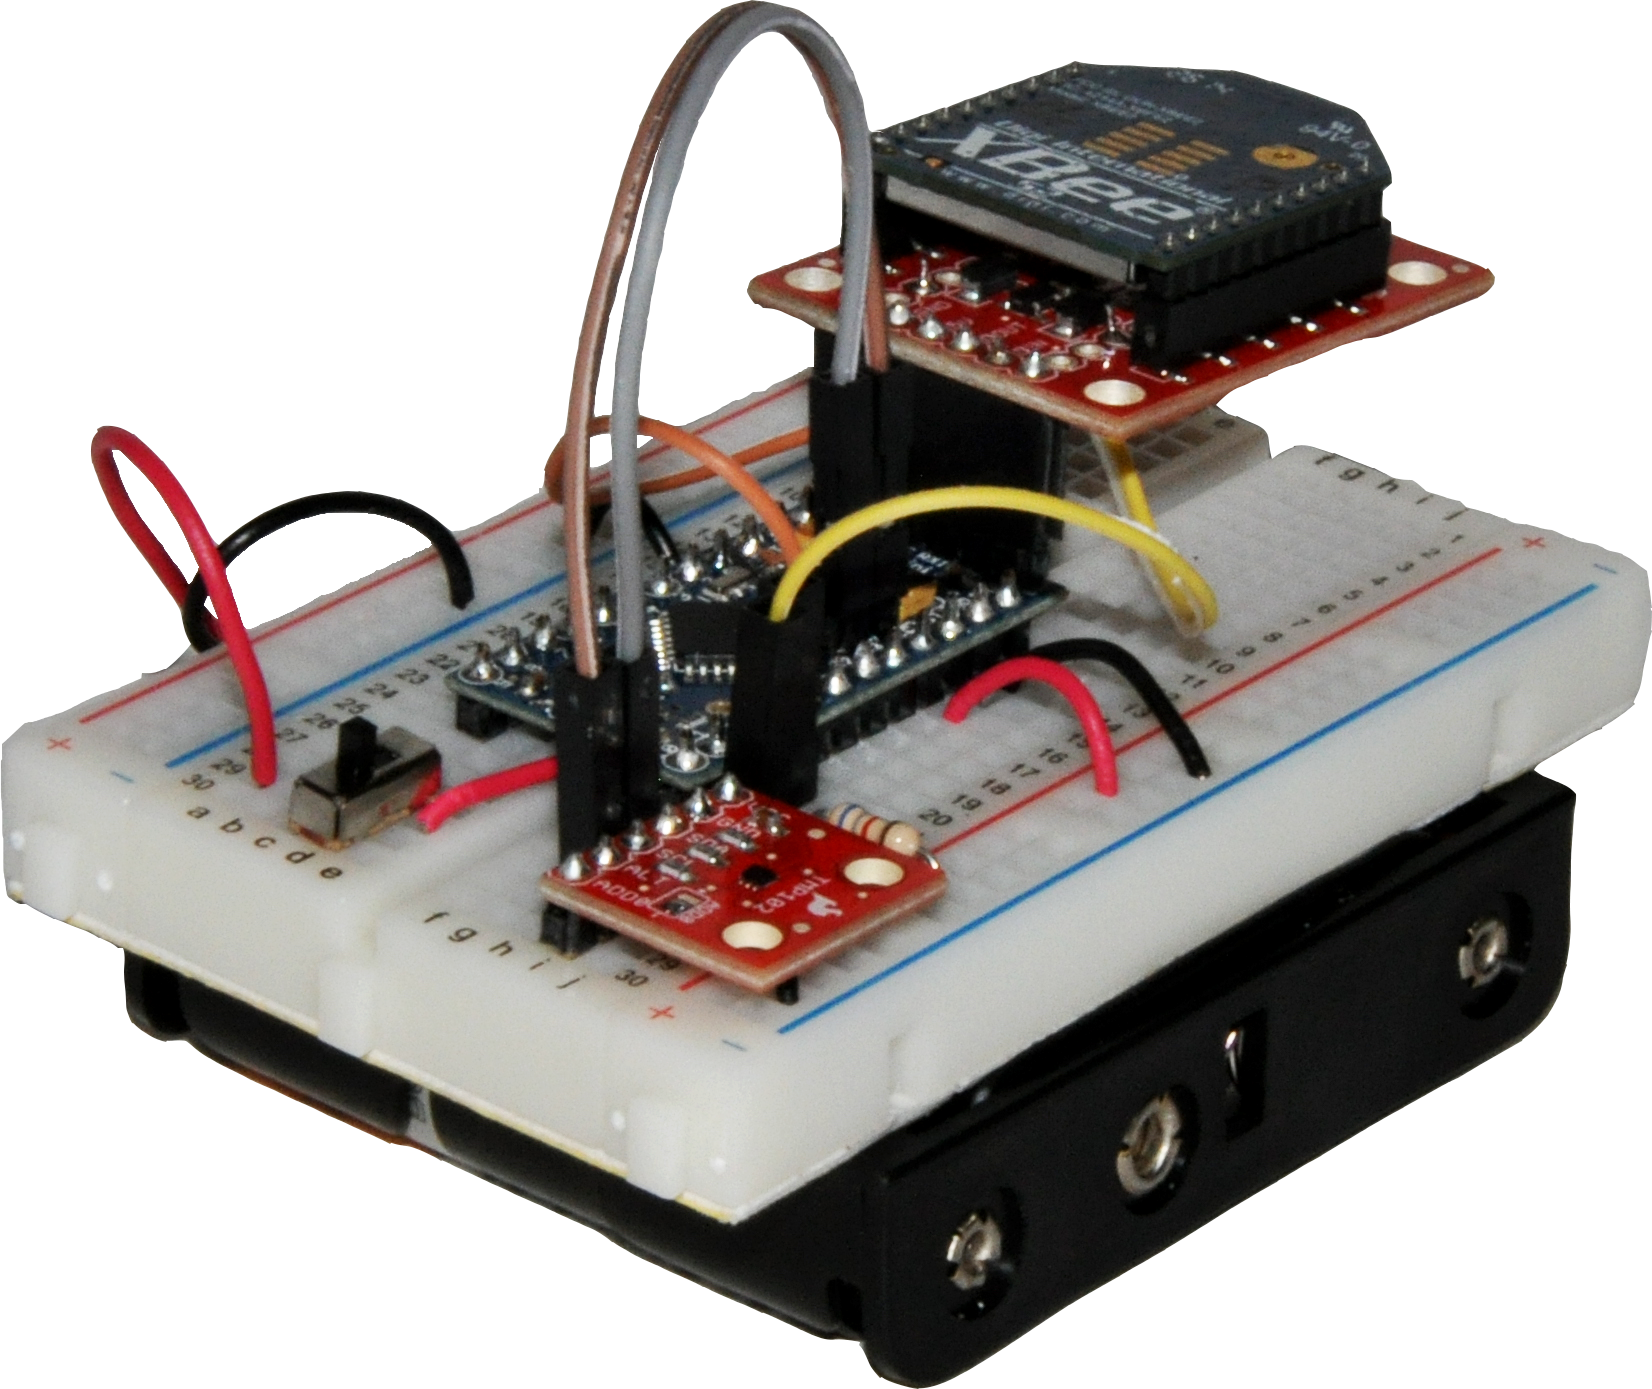
\includegraphics[width=0.6\textwidth]{assets/temp-prototype.png}};
          \end{tikzpicture}
        \caption{Prototype temperature device}\label{figure:temp-device}
      \end{figure}

      \begin{figure}
        \centering
          \begin{tikzpicture}
            \node[inner sep=0pt] at (0,0)
              {\includegraphics[width=0.8\textwidth]{assets/led-prototype.png}};
          \end{tikzpicture}
        \caption{Prototype RGB LED output device}\label{figure:led-device}
      \end{figure}

    \subsection{Bridge}
      The final piece for the complete implementation is the bridge device. Like the end devices, the hardware for this had to first be built. When sourcing the Raspberry Pi devices for this component an additional component, the RPi HAT prototype board was found. Rather than connecting the RPi to the XBee chip with simple wires, this prototype board was used to build a more professional prototype. The RPi HAT required additional soldering, namely the headers to connect it to the RPi, all circuit wires and the XBee Explorer pins. It should also be noted that the Raspberry Pi model B+ (RPiB+)  was procured rather than the model 2 and this was down to its cheaper cost. The RPiB+ is less powerful with a single-core 700MHz processor and 512MB RAM, but is still expected to be sufficiently powerful. The completed hardware can be seen in Figure \ref{figure:bridge-device}.

      As planned, the RPi-maintained distribution of Linux was installed on the RPiB+. A small Node.js application was developed. It made use of the same JavaScript packages which have been implemented in the Haar Engine and Dashboard. One additional role which the application played was to expand on the Compressed JSON Object data format described in the previous section so it could be submitted to Haar API.

      \begin{figure}
        \centering
          \begin{tikzpicture}
            \node[inner sep=0pt] at (0,0)
              {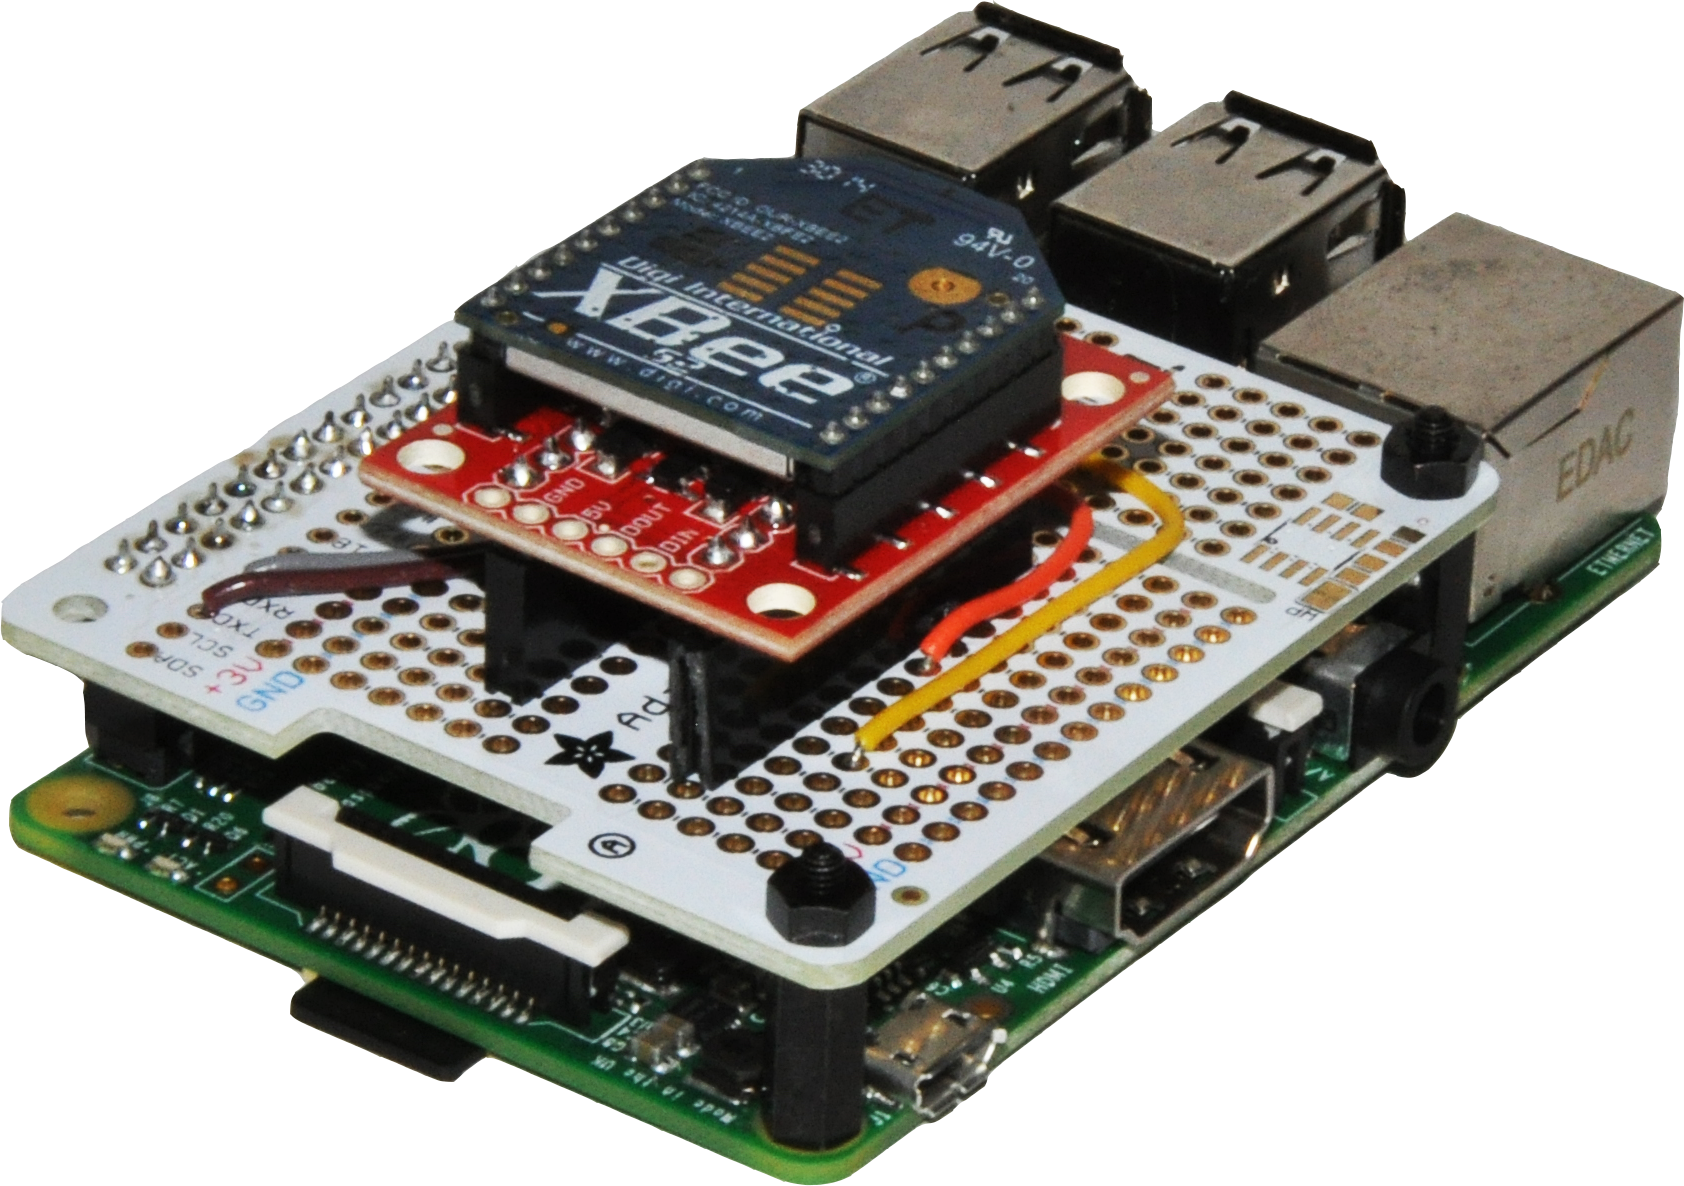
\includegraphics[width=0.6\textwidth]{assets/bridge-prototype.png}};
          \end{tikzpicture}
        \caption{Prototype bridge device}\label{figure:bridge-device}
      \end{figure}
